\chapter{Variational Database Management System (VDBMS)}
\label{ch:vdbms}

%
We implement a prototype using the VDB and VRA frameworks as
%\revised{We implement our VDB and VRA framework as}
\emph{Variational Database Management System (VDBMS)}.
VDBMS is implemented in Haskell. VDBMS sits on 
top of any DBMS that the user used to store their data 
%\arashComment{I did not find any explanation on how variational tables are stored in an RDBMS.} 
%\resp{it is exactly implemented as formalized in variational table section.}
%\responded
in form of variational tables, explained in \secref{vtab}, with one exception:
%However, 
we encode variation at the content level by storing tuples presence condition 
as a presence condition attribute to all tables
since relational databases cannot represent annotations. 
Note that the rest of the presence conditions are stored in the Haskell side of the system.
%To acquire an extensible system we implement 
To support running VDBMS with multiple different plain relational DBMS backends,
we provide
a shared interface
for communicating with the backend DBMS and
%connecting to and inquiring information from a DBMS and
instantiate it for different database engines such as PostgreSQL and
MySQL. 
%\rewrite{any dbms that has a library in haskell that has a function
%that returns the result to the user. eg that doesn't satisfy this is 
%database.sqlite3. } --> The following addresses this:
An expert can extend VDBMS to another database engine by
writing methods for connecting to and querying from the database.

%\input{sections/implVar}
%\point{vdb and vschema and config (bottom of fig).}
\section{VDBMS Architecture}
\label{sec:arch}

\figref{arch} shows the architecture of VDBMS.
% and its modules.
%For now, 
We assume a VDB and its variational schema are generated by an 
expert and are stored in a DBMS.
%, we return to generation of VDBs in 
%\secref{exp-disc}. 
A VDB can be \emph{configured} to its plain relational 
database variants
%, if desired by a user, 
by providing the configuration
of the desired variant, \figref{vdb-conf}.
For example, a SPL developer configures a VDB to produce 
software and its database for a client.
%To configure a VDB, VDBMS requires a list of valid configurations.
%Remember that the feature model is a feature expression that 
%encodes all valid configurations. Hence, solving the feature model
%by a SAT solver results in the list of valid configurations.


\begin{figure}
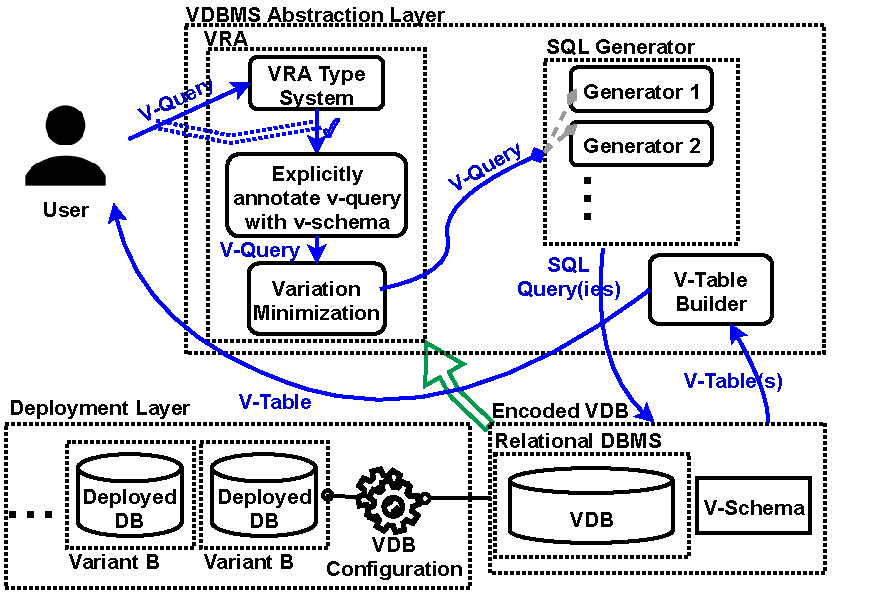
\includegraphics[width = \linewidth] {figs/arch/arch8.pdf}
\caption[VDBMS architecture and execution flow of a variational query]{VDBMS architecture and execution flow of a variational query. 
The dotted double-line from the input variational query
% to explicitly annotate variational query module
indicates the dependency of passing the variational query to this module
only if it is valid. 
The dashed gray arrows with diamond heads demonstrate
an option for the flow of the variational query. 
%We examine taking different routes
%to evaluate a variational query, resulting in various approaches in \secref{apps}.
The blue filled arrows track the data flow, the green hollow arrows 
indicate an input to a module.}
\label{fig:arch}
\end{figure}


%\point{flow of vq in vdbms.}
%Given a VDB and its variational schema, 
To extract information from a VDB, 
a user inputs a variational query \vQ\ to VDBMS.
%
First, \vQ\ is checked by the \emph{type system}.
%, explained in 
%First, \vQ\ is type-checked by the VRA type system introduced in 
%\secref{type-sys}. 
If the query is ill-typed, the user gets an error explaining what part of the 
query violated the variational schema.
%, shown in \exref{q-violate-sch}.
%\moredet{maybe give an ex of an error user will see! ref to ex of error given
%in \secref{type-sys}}
Otherwise, 
\vQ\ is explicitly annotated by the schema and
%defined in \secref{constrain},
%to ensure variation-preserving property w.r.t. variational schema throughout the execution flow of variational query 
%in the system and then
%
%Then, it 
is passed to the \emph{variation minimization} module,
% introduced in 
%\secref{var-min}, 
to simplify \vQ.
%minimize the variation of \vQ\ and apply
%relational algebra optimization rules. 
%
The simplified query is then sent to the \emph{generator} module where
SQL queries are generated from variational queries by different approaches explained 
in \secref{apps}.
%, \secref{apps} provides three
%approaches for this.
%\TODO{
%\exref{q-flow} in \appref{sql-gen} demonstrates the flow of a variational query through
%VDBMS.}
%\wrrite{have examples for each approaches. of mainly the final sql}

\begin{comment}
To generate runnable queries w.r.t. the underlying DBMS,
the minimized query \ensuremath {\VVal \vQ} is passed to 
the \emph{translate to RA} module that could use either 
configuring or grouping of variational queries, explained in \secref{vra-sem},
to generate RA queries. The generated 
queries are then sent to the \emph{SQL generator} module which generates
SQL queries in various ways from the relational algebra queries, explained
in \secref{sql-gen}.
%\moredet{in app have an ex of all this happening!}
\end{comment}

%\point{vtab builder.}
%Having generated a/multiple SQL query/ies, it/they is/are now run over the underlying 
%VDB.
All generated SQL queries are then executed on the underlying VDB.
% (stored in a DBMS desired by the user). 
 The result could be either 
a variational table or multiple variational tables, depending on the approach chosen by
%the translator to RA and 
the SQL generator. The variational table(s) is passed
to the \emph{variational table builder}
%\dropit{could drop \secref{vtab-build} and explain it here!}
%explained in \secref{vtab-build}, 
to create one variational table that filters out 
duplicate and invalid tuples, shrinks presence conditions, and 
eventually, returns the final variational table to the user.
Note that the variational table builder module uses the accumulation
functions introduced in \secref{accum} in addition to filtering out tuples and 
cleaning a variational table. 


%\input{sections/sqlGen}


\section{SQL Generators}
\label{sec:apps}


%\TODO{if parallel running of queries make a difference add it.}
%
Since VDBMS sits on top of a plain relational DBMS, in order to run
variational queries we must translate them into (sets of) plain relational queries,
that is, \emph{SQL generator} module's task.
These generators also inject the qualifiers of attributes in addition to 
adding the projection of presence condition attributes. We demonstrate this
in \exref{ubf} and \exref{uav}.
Then, VDBMS synthesizes the result into a variational table, that is, 
\emph{variational table builder} module's task.
%
Given an explicitly annotated well-typed variational query \vQ,
%constrained by the schema minimized variation, 
we provide three initial 
approaches to generate SQL query(ies) for \vQ:
\begin{enumerate}
%[wide, labelwidth=!, labelindent=0pt, topsep=1pt]
%\itemsep0em
\item
\emph{Naive Brute Force (\nbf)}:
Configures a variational query \vQ\ for all valid configurations, that is, 
\ensuremath{\forall \config \in \confSet}, translates them to RA queries,
and finally generates SQL queries with renaming all subqueries. The 
SQL queries are sent to underlying DBMS and the results are gathered and
cleaned up in variational table builder module. Here is the flow of how results are generated by 
this approach:
%
\[\vQ \mathrel{\mathop{\rightarrow}^{\mathrm{\eeSem \vQ}}} [ ( \config, \pQ ) ] 
\mathrel{\mathop{\rightarrow}^{\mathrm{\textit{translate}}}_{\mathrm{\textit{to SQL}}}} [ ( \config, \sqlQ ) ]
\mathrel{\mathop{\rightarrow}^{\mathrm{\textit{run}}}_{\mathrm{\textit{queries}}}} \textit{v-tables}
\mathrel{\mathop{\rightarrow}^{\mathrm{\textit{v-table}}}_{\mathrm{\textit{builder}}}} \textit{v-table}
\]
%
%\begin{example}
%\label{eg:nbf}
%\wrrite{write the damn thing}
%\end{example}
%
\item
\emph{Unique Brute Force (\ubf)}:
This approach is just like \nbf\ except that we only generate SQL 
queries for unique RA queries which are the result of configuring the variational query.
That is, it uses the unique variants function \ensuremath{\qGroup \vQ} introduced
in \secref{vraconf}.
%The trick is to attach the condition under which a 
%RA query is valid. This condition is a feature expression generated from
%the set of configurations that configured the variational query into the same RA query, that is,
%\ensuremath{
%\qGroup \vQ = \setDef {\annot \pQ \myOR \forall \config \in \confSet: \fSem \dimMeta = \t,
%\eeSem \vQ = \pQ}
%}. 
The implementation of this function is more efficient than its definition.
%\remember{
%In fact, it follows the function defined in \figref{} in \appref{}.
%}
That is:
%Groups variants of a variational query, translates them to RA queries,
%and generates SQK queries with renaming subqueries. Similar to 
%\ensuremath{(1)} results are gathered and cleaned up by variational table builder module.
%Here is the flow of how results are generated by 
%this approach:
%
\[\vQ \mathrel{\mathop{\rightarrow}^{\mathrm{\qGroup \vQ}}} [ \annot [\dimMeta] {\pQ} ] 
\mathrel{\mathop{\rightarrow}^{\mathrm{\textit{translate}}}_{\mathrm{\textit{to SQL}}}} [ \annot [\dimMeta] {\sqlQ} ]
\mathrel{\mathop{\rightarrow}^{\mathrm{\textit{run}}}_{\mathrm{\textit{queries}}}} \textit{v-tables}
\mathrel{\mathop{\rightarrow}^{\mathrm{\textit{v-table}}}_{\mathrm{\textit{builder}}}} \textit{v-table}
\]
%
\begin{example}
\label{eg:ubf}
Consider query $\vQ_1 = \pi_{\optAtt [\vFour \vee \vFive] [\empno], \name, \fname, \lname} (\empbio)$ given in \exref{vq-specific}. Its corresponding SQL queries generated by either \nbf\ or \ubf\ 
that will eventually be run on the
database and their corresponding feature expression indicating the valid group of configurations are
given below.
For configurations \setDef {} and \setDef {\vThree}
(indicated by the feature expression $(\neg \vThree \wedge \neg \vFour \wedge \neg \vFive) \vee 
(\vThree \wedge \neg \vFour \wedge \neg \vFive)$) we have the query:
%
\begin{lstlisting}[basicstyle=\footnotesize\ttfamily,columns=flexible,lineskip=0.5\baselineskip]
SELECT NULL
\end{lstlisting}
%
For configuration \setDef {\vFour} (indicated by the feature
express $\neg \vThree \wedge \vFour \wedge \neg \vFive$) we have the query:
%
\begin{lstlisting}[basicstyle=\footnotesize\ttfamily,columns=flexible,lineskip=0.5\baselineskip]
SELECT empno, 
        name,
        CONCAT( '(', t0.prescond, ')') AS prescond
FROM v_empbio AS t0
\end{lstlisting}
%
And finally, for configuration \setDef {\vFive} (indicated 
by the feature expression $\neg \vThree \wedge \neg \vFour \wedge \vFive$) we have the
query:
%
\begin{lstlisting}[basicstyle=\footnotesize\ttfamily,columns=flexible,lineskip=0.5\baselineskip]
SELECT empno,
        firstname, 
        lastname,
        CONCAT( '(', t0.prescond, ')') AS prescond
FROM v_empbio AS t0
 \end{lstlisting}
%
Note that the only difference between \nbf\ and \ubf\ is that the former uses configurations
and assigns them to SQL queries and then gathers their tables into a variational tables 
whereas the latter uses the feature expressions indicating a group of configuration and
assigns them to  SQL queries and then gathers their tables into a variational tables. 
For example, \nbf\ uses the configurations given in this examples and runs the first SQL
query twice whereas \ubf\ uses the feature expressions and thus, runs each SQL only 
once. This does not have a big impact as long as the query is an empty query but it would
be less efficient otherwise.
\end{example}
%
\item
\emph{Union-All-Variants (\uav)}:
This approach takes the SQL queries generated by \ubf\ and 
unions them to just run one SQL query. In order to do so it 
forces all the SQL queries to return the same relation schema.
%return the same set of attributes.
Additionally, it applies the presence condition of a SQL query
to its tuples by concating it with the presence condition attribute
in the projected attribute set.
%Groups variants of a variational query, translates them to RA queries, 
%translates RA queries to SQL queries, 
%%generates one SQL query from all SQL queries by u
%unifies the set of
%attributes returned by SQL queries (by getting all returned attributes from
%the type of the variational query and for an attribute \vAtt\ that a SQL query is not returning,
%it uses \ensuremath{\mathbf{NULL} \textit{\ } \mathbf{AS} \textit{\ } \vAtt} syntax),
%attaches the presence condition of variant SQL queries to them (by concating the
%feature expression with presence condition attribute in the returned attribute set),
%%, i.e., 
%%\ensuremath{\mathbf{presenceCond} \textit{\ }  
%and finally combines SQL queries by set operation union. 
The query is sent to the underlying
DBMS and the result is cleaned up by the variational table builder. Finally, it is 
returned to the user as a variational table. Note that cleaning up
the result is part of variational table builder tasks.
%% by attaching presence 
%%condition of attributes to them. 
%Here is the flow of how results are generated by 
%this approach:
That is:
%
\[\vQ \mathrel{\mathop{\rightarrow}^{\mathrm{\qGroup \vQ}}} [ \annot [\dimMeta] {\pQ} ] 
\mathrel{\mathop{\rightarrow}^{\mathrm{\textit{generate}}}_{\mathrm{\textit{SQL}}}} [ \annot [\dimMeta] {\sqlQ} ]
\mathrel{\mathop{\rightarrow}^{\mathrm{union}}} {\VVal \sqlQ}
\mathrel{\mathop{\rightarrow}^{\mathrm{\textit{run}}}_{\mathrm{\textit{query}}}} \textit{v-table}
%\mathrel{\mathop{\rightarrow}^{\mathrm{\textit{clean up}}}} \textit{v-table}
\]
%
\begin{example}
\label{eg:uav}
Consider query $\vQ_1 = \pi_{\optAtt [\vFour \vee \vFive] [\empno], \name, \fname, \lname} (\empbio)$ 
introduced in \exref{vq-specific}. The final SQL query generated by the \uav\ approach is:
 \begin{lstlisting}[basicstyle=\footnotesize\ttfamily,columns=flexible,lineskip=0.5\baselineskip]
 (SELECT empno,
          firstname,
          lastname,
          NULL AS name,
          CONCAT( '(', t0.prescond, ')', ') AND ('
                 , '(NOT v3 AND v4) AND NOT v5'
                 , ')') AS prescond,
  FROM empbio AS t0) 
UNION ALL 
 (SELECT empno,
          NULL AS firstname,
          NULL AS lastname,
          name,
          CONCAT( '(', t1.prescond, ')', ') AND ('
                 , '(NOT v3 AND NOT v4) AND v5'
                 , ')') AS prescond
  FROM empbio AS t1)
 \end{lstlisting}
%
\end{example}
%
\item 
\emph{Injected Naive Brute Force (\nbfi)}: 
Alternatively, the feature expression associated with a configuration can be injected
inside the SQL query. Thus, simplifying the variational table builder to just fix the 
schema of the returned tables. \exref{ubfi} illustrates this approach. 
%
\item 
\emph{Injected Unique Brute Force (\ubfi)}:
Similarly, the injection of feature expressions into the SQL queries can be applied to
the \ubf\ approach. \exref{ubfi} illustrates this approach.
%
\begin{example}
\label{eg:ubfi}
Employing the \nbfi\ or \ubfi\ approaches to the query $\vQ_1$ results in the following SQL queries.
For configuration \setDef {\vFour} (indicated by the feature
express $\neg \vThree \wedge \vFour \wedge \neg \vFive$) we have the query:
%
\begin{lstlisting}[basicstyle=\footnotesize\ttfamily,columns=flexible,lineskip=0.5\baselineskip]
SELECT empno, 
        name,
        CONCAT( '(', t0.prescond, ')', ') AND ('
               , '(NOT v3 AND v4) AND NOT v5'
               , ')') AS prescond,
FROM v_empbio AS t0
\end{lstlisting}
%
For configuration \setDef {\vFive} (indicated 
by the feature expression $\neg \vThree \wedge \neg \vFour \wedge \vFive$) we have the
query:
%
\begin{lstlisting}[basicstyle=\footnotesize\ttfamily,columns=flexible,lineskip=0.5\baselineskip]
SELECT empno,
        firstname, 
        lastname,
        CONCAT( '(', t0.prescond, ')', ') AND ('
               , '(NOT v3 AND NOT v4) AND v5'
               , ')') AS prescond
FROM v_empbio AS t0
 \end{lstlisting}
%
\end{example}
\end{enumerate}

We use the first two methods
%SQL generators 
to simulate existing approaches used to manage
variation currently. In particular, \nbf\ simulates how a naive
DBA would conduct such a task. \ubf\ simulates
how an expert DBA would conduct such a task. 
\uav\ attempts to reuse as much of the already existing results as possible. 
%
The generated SQL queries need to be independent from the 
underlying DBMS that stores the VDB. Hence, the SQL generator module
has a submodule that prints generated SQL queries for each DBMS engine. 


%add this somewhere: -> check that you have this in use cases
%We implemented these checks in our VDBMS tool and verified that both use cases
%described in this paper satisfy all of them. 
To ensure that these methods are implemented correctly we conducted two
sanity checks:
\begin{enumerate}
\item We check that the variation-preserving property at the semantics level
holds for all the methods. That is, we check that configuring the result gotten from
a method is the same as running the configured query over the corresponding 
configured database.
%
\item We check that the results from each two methods are equivalent based on
the equivalency relation over variational sets defined in \secref{vset} 
(specifically, in \secref{vset}).
\end{enumerate}

Our set of queries for both the email VDB and employee VDB passed these sanity checks.

\section{Experiments}
\label{sec:exp}

\wrrite{write the damn thing.}



